% This is samplepaper.tex, a sample chapter demonstrating the
% LLNCS macro package for Springer Computer Science proceedings;
% Version 2.20 of 2017/10/04
%
\documentclass[runningheads]{llncs}
%
\usepackage{graphicx}
\graphicspath{{./images/}}
% Used for displaying a sample figure. If possible, figure files should
% be included in EPS format.
%
% If you use the hyperref package, please uncomment the following line
% to display URLs in blue roman font according to Springer's eBook style:
% \renewcommand\UrlFont{\color{blue}\rmfamily}

\begin{document}
%
\title{LightBulbs - Constraint Logic Programming}
%
%\titlerunning{Abbreviated paper title}
% If the paper title is too long for the running head, you can set
% an abbreviated paper title here
%
\author{Ivo Saavedra - up201707093\and
João Cardoso - up201806531 \\
\small{FEUP-PLOG, 3MIEIC01, Grupo LightBulb}}

%
\authorrunning{F. Author et al.}
% First names are abbreviated in the running head.
% If there are more than two authors, 'et al.' is used.
%
\institute{Faculdade de Engenharia da Universidade do Porto, Rua Roberto Frias, 4200-465 Porto, Portugal}
%
\maketitle              % typeset the header of the contribution
%
\begin{abstract}
This article contains the implementation details of the application developed for the second assignment for the
Logical Programming subject. The goal of this project was to develop a program capable of creating and solving every instance of the Light bulb puzzle. The goal of this puzzle is to find every lit light bulb, considering that a light bulb is only lit if and only if the number inside it is equal to the number of lit neighboring lamps (including itself).

\keywords{PROLOG  \and SICStus \and Lightbulbs.}
\end{abstract}
%
%
%
\section{Introduction}
This article was developed as complement for the second partical assignment of the Logical Programming subject of the 3rd year of the MIEIC course. The goal of this project was to develop an application capable of creating and solving "Lightbulb" type puzzles using the SISCstus prolog development system along with the restriction tools provided by the CLPFD library. The objective of these puzzles is to determine which light bulbs inside a n*n square are turned on. A light bulb is only on when the number of adjacent bulbs (including itself) equals the number attributed to it. This document is organized in the following manner:
	\begin{itemize}
		\item[•] \textbf{Problem Description:} detailed description of the problem being analyzed
		\item[•] \textbf{Approach:} section describing the implementation of the application
		\begin{itemize}
			\item[-] \textbf{Decision Variables:} description of the decision variables and their domains
			\item[-] \textbf{Constraints:} details of the rigid and flexible constraints
		\end{itemize}
		\item[•] \textbf{Solution Presentation:} description of the adopted solution presentation
		\item[•] \textbf{Experiments and Results:}
		\begin{itemize}
			\item[-] \textbf{Dimension Analysis:} results obtained after testing boards of different sizes
			\item[-] \textbf{Search Strategies:} result comparison of different heuristics search functions
		\end{itemize}
		\item[•] \textbf{Conclusions}
		\item[•] \textbf{References}
	\end{itemize}

\section{Problem description}
The Lightbulb puzzle consists of a two dimensonal board consisting of n[1*] light bulbs per line and m[1*] light bulbs per column, where each lightbulb has a number on it.
Each lightbulb is on if and only if it's number is equal to the number of lit neighboring (directly or diagonally adjacent) lightbulbs, including itself. When given a board we must determine all it's possible solutions; the number of solutions may range from one to many, however there are cases in which the board is impossible to solve. Having that in consideration we classified the LightBulbs puzzle as a decision problem.

\section{Approach}

\subsection{Decision Variables}
For this puzzle the decision variables are the values inside each cell of the input board. As previously stated, each board cell as a value representing the number of adjacent bulbs that need to be lit in order for the current cell to be as well.
Taking into consideration that every cell can at most have eight adjacent cells and that for the bulb to be lit we need to have N adjacent lit bulbs plus the current one we come to the conclusion that the maximum number inside a light bulb is 8+1=9. As for the minimum value we came to the conclusion that it should be 1. If the value inside a bulb was equal to zero, then that bulb would always be turned off, because of the constraints of this puzzle.

\subsection{Constraints}
As previously mentioned, a bulb is only lit when the number inside it is equal to the number of adjacent light bulbs (including itself) that are lit. In order to accomplish this we iterated over all of the input board's cells and for each cell we fetched every adjacent variable. The maximum number of adjacent cells is eight, so for each light bulb we needed eight variables. If the current cell had less than eight neighbors, for instance, if it was in a corner, then the adjacent variables that were out of bounds would take the value of zero.
After having gotten all the adjacent variables we started applying the constraints. The first one being that the sum of all the adjacent variables should be different from the number inside the current bulb 
(TODO: EXPLAIN)

\clearpage
\section{Solution Presentation}
In order to make the solution more intelligible, the input board is displayed along with the result board, in which the latter
only contains the cells that have a lit bulb, allowing for an easier understanding of the solution. The elapsed time is also displayed for the experiments and results section.
The predicates responsible for displaying the results are called after the solution is obtained. As each board can originate more than one result the solution consists of a list of matrices, each one representing the possible output boards for the original board. The \textbf{showResults} predicate is responsible for iterating over the result matrices and displaying each one in the console.

\begin{figure}[h]
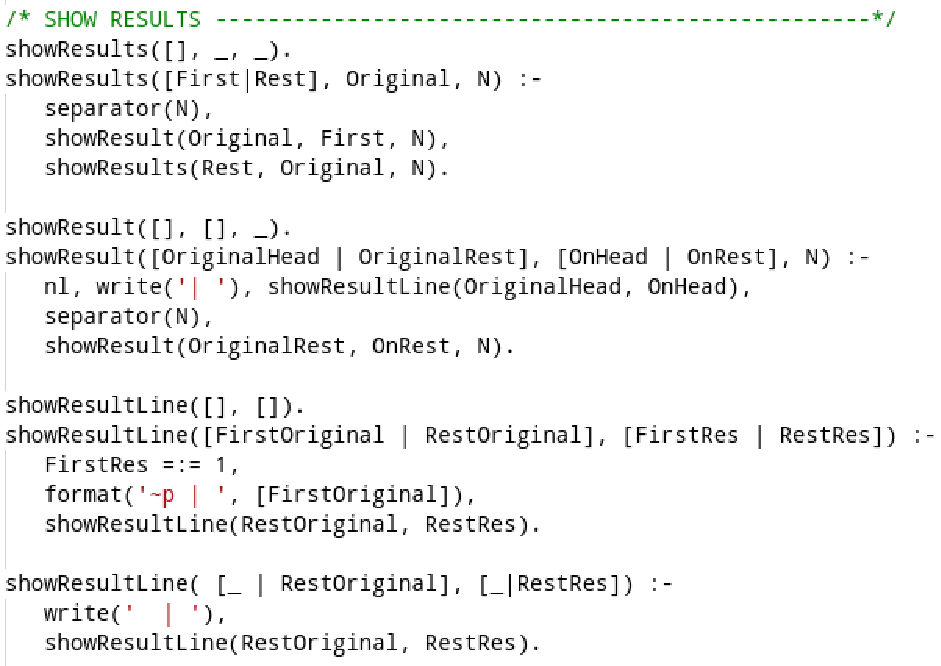
\includegraphics[scale=0.5]{showResults}
\centering
\caption{display result predicates}
\centering
\vspace{5mm}	
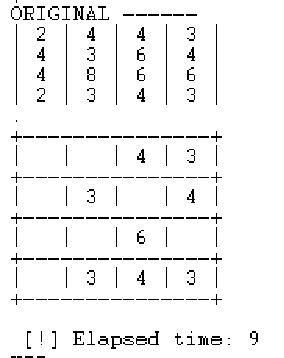
\includegraphics[scale=1]{solutionDisplay}
\centering
\caption{solution display example}
\centering
\end{figure}

\section{Experiments and Results}
\subsection{Dimension Analysis}
\subsection{Search Strategies}

\section{Conclusions}
The objective of this project was to develop an application capable of creating and solving light bulb puzzles. At the end of this assignment we feel that our knowledge on the CLPFD prolog module has definitely increased as well as our experience with constraint logical programming.



\section{References}

% ---- Bibliography ----
%
% BibTeX users should specify bibliography style 'splncs04'.
% References will then be sorted and formatted in the correct style.
%
% \bibliographystyle{splncs04}
% \bibliography{mybibliography}
%
\begin{thebibliography}{8}
\bibitem{ref_article1}
Author, F.: Article title. Journal \textbf{2}(5), 99--110 (2016)

\bibitem{ref_lncs1}
Author, F., Author, S.: Title of a proceedings paper. In: Editor,
F., Editor, S. (eds.) CONFERENCE 2016, LNCS, vol. 9999, pp. 1--13.
Springer, Heidelberg (2016). \doi{10.10007/1234567890}

\bibitem{ref_book1}
Author, F., Author, S., Author, T.: Book title. 2nd edn. Publisher,
Location (1999)

\bibitem{ref_proc1}
Author, A.-B.: Contribution title. In: 9th International Proceedings
on Proceedings, pp. 1--2. Publisher, Location (2010)

\bibitem{ref_url1}
LNCS Homepage, \url{http://www.springer.com/lncs}. Last accessed 4
Oct 2017
\end{thebibliography}
\end{document}
